\documentclass[10pt]{article}

\usepackage[colorlinks, linkcolor=red, urlcolor=blue]{hyperref}
\usepackage{graphicx}

\title{
    {\normalsize Paper Note} \\
    {\large \href{https://openaccess.thecvf.com/content_CVPR_2020/papers/Wang_Semi-Supervised_Learning_for_Few-Shot_Image-to-Image_Translation_CVPR_2020_paper.pdf}{Semi-supervised Learning for Few-shot Image-to-Image Translation
    }} \\
    {\normalsize Project Link: \href{https://github.com/yaxingwang/SEMIT}{Github}}
}

\begin{document}
    \maketitle

    \section{Background}
        \subsection*{Previous Work}
            \begin{itemize}
                \item \href{https://arxiv.org/pdf/1806.06029.pdf}{one-shot I2I translation by first training a variational autoencoder for the seen domain and then adapting those layers related to the unseen domain.}
                \item \href{https://arxiv.org/pdf/1906.00184.pdf}{zero-shot I2I translation, employ- ing the annotated attributes of unseen categories instead of the labeled images.}
                \item \href{https://arxiv.org/pdf/1905.01723.pdf}{few-shot I2I translation in a multi-class setting. These models, however, need to be trained using large amounts of hand-annotated ground-truth labels for images of the source domain}
            \end{itemize} 

        \subsection*{Limitations}
            Labeling large-scale datasets is costly and time consuming, making those methods less applicable in practice. 
            In this paper, they overcome this limitation and explore a novel setting, few-shot I2I translation
            in which only limited labeled data is available from the source classes during training. \\
        
            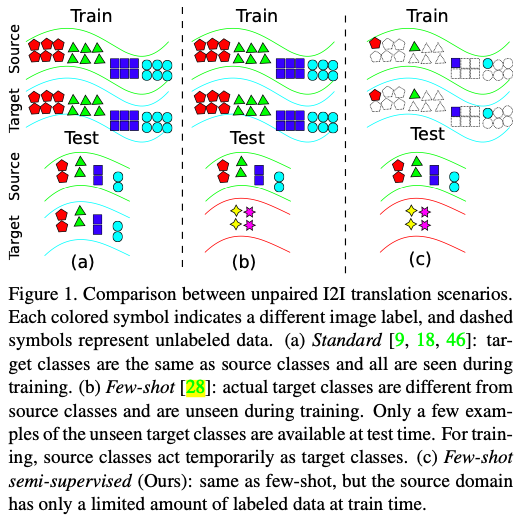
\includegraphics[width=\linewidth]{src/img/Comparison between unpaired I2I translation scenarios.png} \\



\end{document}